\documentclass[12pt]{article}

% Correção para erro \normalsfcodes no Overleaf / TeX Live 2025
\makeatletter
\DeclareRobustCommand{\normalsfcodes}{%
  \sfcode`\.=3000
  \sfcode`\?=3000
  \sfcode`\!=3000
  \sfcode`\:=2000
  \sfcode`\;=1500
  \sfcode`\,=1250
}
\makeatother

\usepackage{sbc-template}
\usepackage{graphicx,url}
\usepackage[utf8]{inputenc}
\usepackage[T1]{fontenc}
\usepackage[brazil]{babel}
\usepackage{booktabs}
\usepackage{tabularx}
\usepackage{array}
\usepackage[hidelinks]{hyperref}

\sloppy

\title{Uma Arquitetura DataOps Orientada a Eventos para Processamento de Dados Geoespaciais em Tempo Real}

\author{Gabriel Gonçalves Sampaio\inst{1}, Barbara Pimenta Caetano\inst{1}}

\address{Instituto de Engenharia de Sistemas e Tecnologia da Informação (IESTI) \\
  Universidade Federal de Itajubá (UNIFEI)\\
  Avenida BPS, 1303 -- 37500-903 -- Itajubá -- MG -- Brasil
  \email{gabrielsampaio059@gmail.com, bpimentacaetano@unifei.edu.br}
}

\begin{document}

\maketitle

\begin{abstract}
  The growing demand for real-time geospatial data processing poses challenges related to the ingestion, storage, and continuous analysis of large volumes of information. This paper presents an event-driven DataOps architecture designed to continuously integrate the stages of collection, spatial clustering, and topological modeling of geographic data. The architecture comprises a messaging system for data stream ingestion, an in-memory spatial indexing structure, and a columnar database for analytical storage. For validation, the platform was applied to wildfire hotspot monitoring, integrating Spatio-Temporal Density-Based Spatial Clustering (ST-DBSCAN) to track dynamic fire events, and Network Science (Betweenness Centrality) to evaluate cascade failure risks in the Brazilian National Interconnected System (SIN). The results demonstrate the capability to group raw hotspots into unified fire events and identify critical power substations with high processing stability, indicating that the proposed architecture is suitable for advanced continuous geospatial intelligence.
\end{abstract}

\begin{resumo}
  A crescente demanda por processamento de dados geoespaciais em tempo real impõe desafios na ingestão, armazenamento e modelagem analítica contínua de grandes volumes de informação. Este trabalho apresenta uma arquitetura DataOps orientada a eventos, projetada para integrar de forma contínua a coleta, o processamento e a orquestração de dados espaciais. A arquitetura é composta por sistemas de mensageria (Kafka), indexação espacial em memória (R-Tree/KDTree), armazenamento colunar (Druid) e orquestração (Dagster). Para validação, a plataforma foi aplicada ao monitoramento de incêndios, integrando clusterização baseada em densidade espaço-temporal (ST-DBSCAN) para transmutar focos pontuais em eventos dinâmicos (polígonos), além do emprego de Ciência de Redes para avaliar riscos de falha em cascata no Sistema Interligado Nacional (SIN). Os resultados obtidos em um ambiente com recursos computacionais limitados demonstram estabilidade na ingestão, eficiência no armazenamento e a capacidade de mapear vulnerabilidades em infraestruturas críticas, indicando que a arquitetura proposta é adequada para cenários que exigem processamento geoespacial contínuo.
\end{resumo}

\section{Introdução}

O mercado atual de dados exige que informações sejam coletadas, processadas e entregues em intervalos cada vez menores. Em áreas como meio ambiente e energia, o valor do dado depende da velocidade com que ele se torna útil para apoiar decisões. Nesse cenário, não basta armazenar grandes volumes de dados, é necessário transformá-los em informações confiáveis e contextualizadas.

Essa necessidade é ainda mais evidente em dados geoespaciais. Uma coordenada térmica isolada informa apenas uma anomalia pontual, não elucidando a propagação de um incêndio florestal ou o impacto imediato sobre a rede elétrica. Para que um evento espacial seja útil, é necessário conectá-lo ao território, considerando infraestrutura próxima, serviços disponíveis e áreas protegidas.

Este trabalho aplica essa lógica ao monitoramento de focos de incêndio. Os dados do Programa Queimadas do Instituto Nacional de Pesquisas Espaciais (INPE) indicam eventos térmicos detectados por satélite \cite{inpe_queimadas}. Quando estes vetores térmicos são submetidos a algoritmos de clusterização de densidade espaço-temporal (ST-DBSCAN), é possível rastrear o ciclo de vida contínuo de um grande incêndio. Adicionalmente, cruzando estes eventos com a infraestrutura do Operador Nacional do Sistema (ONS) modelada via teoria de grafos, viabiliza-se o cálculo do risco de impactos em infraestruturas vitais.

Dessa forma, este artigo apresenta uma evolução de uma arquitetura DataOps orientada a eventos para processamento geoespacial em tempo real. A proposta integra Apache Kafka para mensageria \cite{apache_kafka}, Apache Druid para persistência analítica \cite{apache_druid}, Apache Superset para visualização \cite{apache_superset} e o Apache Dagster para a orquestração formal de pipelines.

\section{Revisão Bibliográfica}

Arquiteturas modernas de dados buscam reduzir a latência entre a coleta, o processamento e a disponibilização da informação. O conceito de DataOps propõe a aplicação de práticas de automação, rastreabilidade, integração contínua e orquestração determinística ao ciclo de vida dos dados \cite{ereth2018dataops}. Essas práticas são fundamentais em pipelines que exigem validação constante e entrega confiável para análise.

Em ambientes analíticos geoespaciais, a transformação de eventos observacionais brutos em dimensões enriquecidas requer a aplicação de modelos dimensionais organizados em tabelas fato e dimensões, facilitando consultas e agregações \cite{kimball2013}.

Do ponto de vista preditivo, a análise de eventos dinâmicos como incêndios exige extrapolar a análise pontual. O algoritmo ST-DBSCAN estende a clusterização baseada em densidade ao incorporar a dimensão temporal, viabilizando o agrupamento de pontos contíguos no espaço e no tempo \cite{birant2006stdbscan}. Simultaneamente, a estabilidade de infraestruturas conectadas é amplamente estudada pela Ciência de Redes. A Centralidade de Intermediação (\textbf{Betweenness Centrality}) atua como um previsor confiável de gargalos em grafos complexos, como malhas de transmissão de alta tensão \cite{freeman1977set}.

\section{Arquitetura DataOps Proposta}

A arquitetura foi organizada em etapas independentes: orquestração, preparação das bases, processamento espacial, mensageria e persistência analítica. O ecossistema é alicerçado sobre uma base de processamento de fluxos desenhada para alinhar baixa latência com consultas rápidas (Figura \ref{fig:streaming}).

\begin{figure}[htpb]
    \centering
    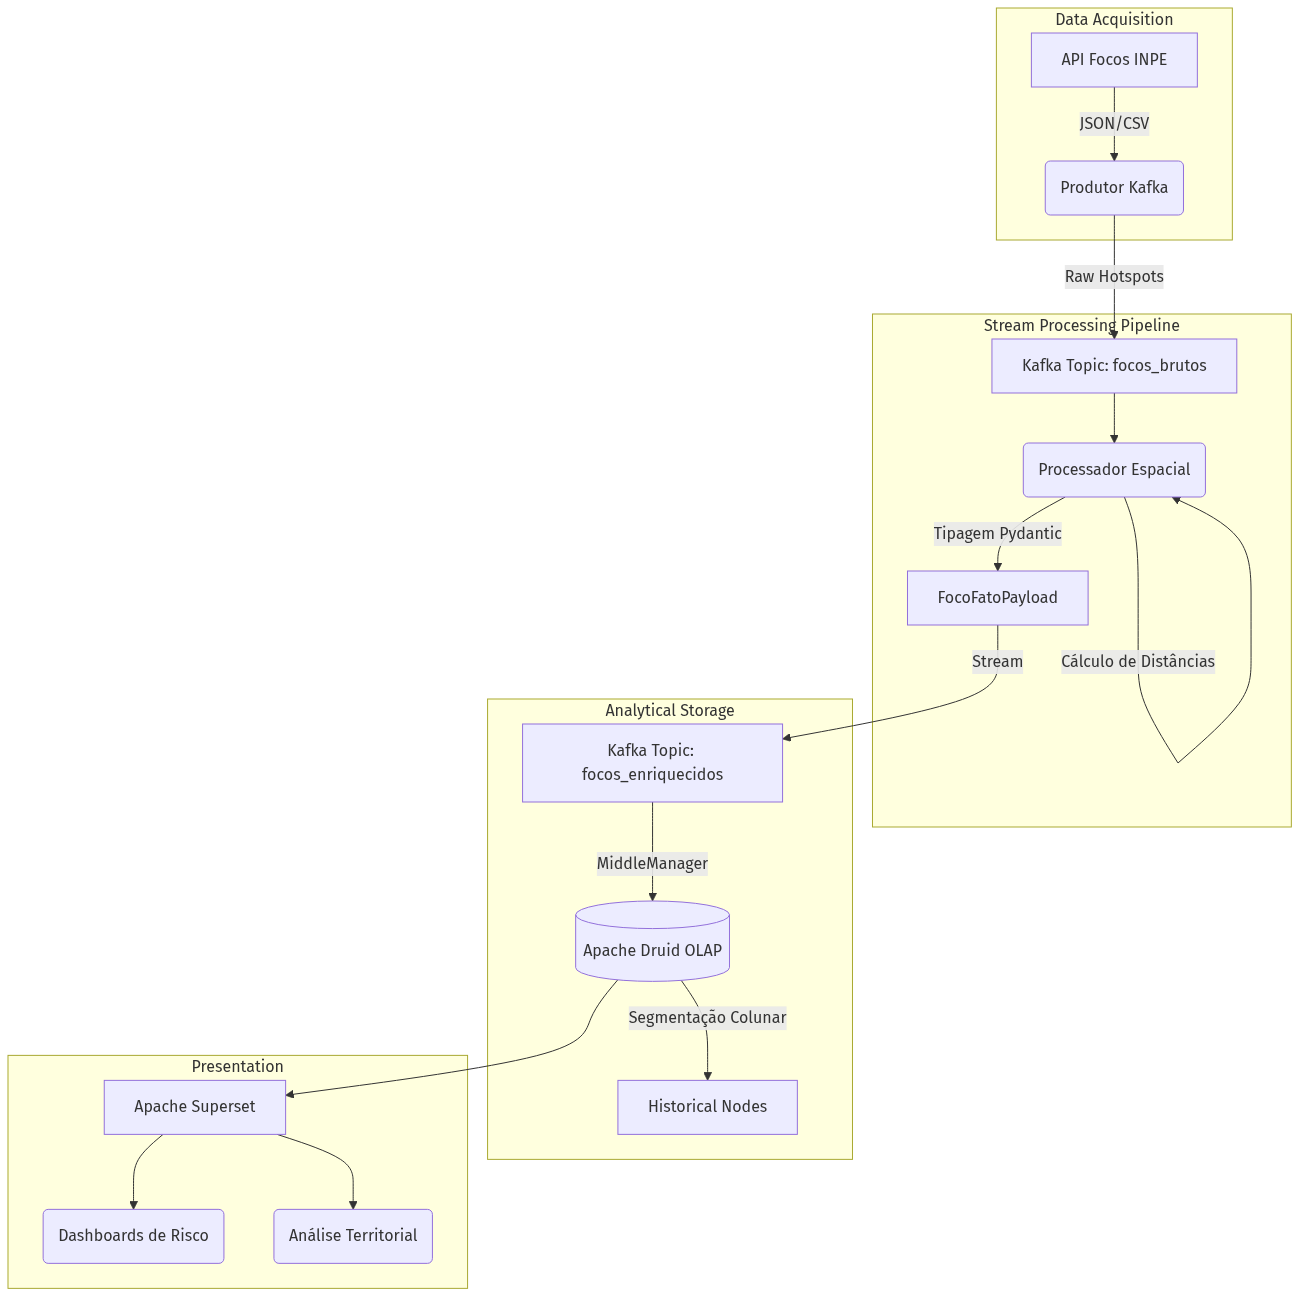
\includegraphics[width=0.9\textwidth,height=0.35\textheight,keepaspectratio]{diagrama_streaming.png}
    \caption{Topologia de Streaming e Armazenamento Analítico.}
    \label{fig:streaming}
\end{figure}

O fluxo de dados opera com múltiplas fontes: dados estáticos (municípios, infraestrutura do ONS, DNIT e FUNAI) e APIs de tempo real (focos do INPE). A ingestão funde esses universos distintos sob o mesmo pipeline. O módulo de processamento espacial não persiste estados, apenas intercepta os dados brutos, sobrepõe as geometrias usando indexação espacial (R-Tree/KDTree) e injeta cálculos de distância contínua.

Cada evento enriquecido é enviado ao Kafka, que desacopla a produção dos dados da ingestão analítica. O Apache Druid consome esse fluxo e armazena os eventos em formato colunar. Seguindo o modelo dimensional, o pacote de dados descarta atributos textuais extensos (como nomes de municípios), retendo na tabela fato apenas as chaves primárias e métricas puras, delegando a reconstrução textual ao Apache Superset em tempo de consulta.

\subsection{Orquestração Declarativa (Dagster)}

Para garantir a rastreabilidade e a correta execução das etapas, a governança do projeto foi integralmente delegada ao framework Apache Dagster. Os scripts matemáticos e motores ETL foram modelados como \textbf{Software-Defined Assets} (Figura \ref{fig:dagster}).

\begin{figure}[htpb]
    \centering
    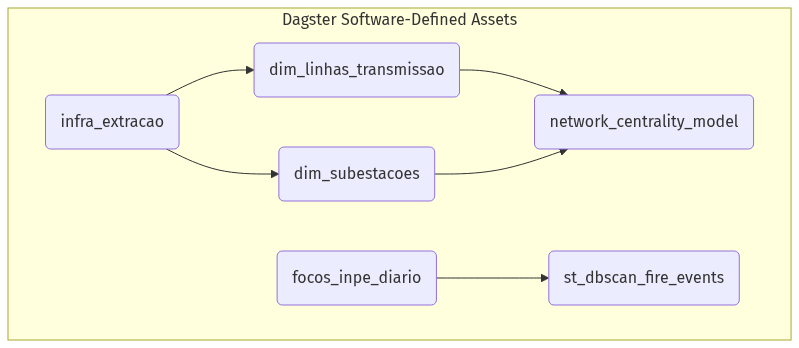
\includegraphics[width=0.9\textwidth,height=0.35\textheight,keepaspectratio]{diagrama_dagster.png}
    \caption{Grafo de Orquestração DataOps utilizando Dagster.}
    \label{fig:dagster}
\end{figure}

A orquestração cria um Grafo Acíclico Dirigido (DAG) tipado que permite visualizar a linhagem dos dados (\textbf{Data Lineage}). Por exemplo, o script de centralidade de rede depende explicitamente da extração das dimensões do ONS. Essa estrutura elimina a concorrência arbitrária de agendadores simples (como \textit{CRON jobs}), assegurando que as análises geofísicas ocorram apenas após a validação e limpeza prévia dos dados espaciais.

\section{Processamento Espacial e Modelagem Analítica}

\subsection{Clusterização ST-DBSCAN: O Foco como Evento}

A arquitetura evoluiu o tratamento dos focos de incêndio de uma visão de coordenada pontual isolada para o conceito de \textbf{Eventos de Incêndio Dinâmicos} (Figura \ref{fig:dbscan}).

\begin{figure}[htpb]
    \centering
    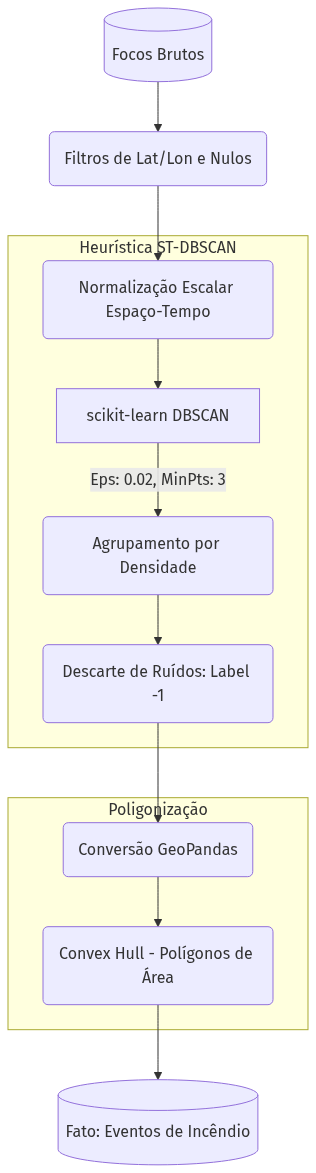
\includegraphics[width=0.9\textwidth,height=0.35\textheight,keepaspectratio]{diagrama_dbscan.png}
    \caption{Fluxo de Clusterização ST-DBSCAN para geração de Eventos Dinâmicos.}
    \label{fig:dbscan}
\end{figure}

Os focos brutos provenientes do satélite passam por um motor que normaliza as grandezas de espaço e tempo. Através do algoritmo ST-DBSCAN, anomalias isoladas são agrupadas considerando a densidade temporal e espacial simultaneamente. Posteriormente, as bibliotecas \textbf{GeoPandas} e \textbf{Shapely} calculam a Envoltória Convexa (\textbf{Convex Hull}) de cada \textit{cluster}, gerando polígonos. Assim, o fogo deixa de ser tratado como um ponto e passa a ser compreendido como uma área afetada com evolução temporal, permitindo o monitoramento do seu perímetro pela defesa civil.

\subsection{Ciência de Redes no SIN (NetworkX)}

O impacto dos incêndios em áreas críticas e o risco de falhas em cascata no Sistema Interligado Nacional (SIN) foram quantificados matematicamente modelando a infraestrutura como um Grafo Complexo (Figura \ref{fig:grafos}).

\begin{figure}[htpb]
    \centering
    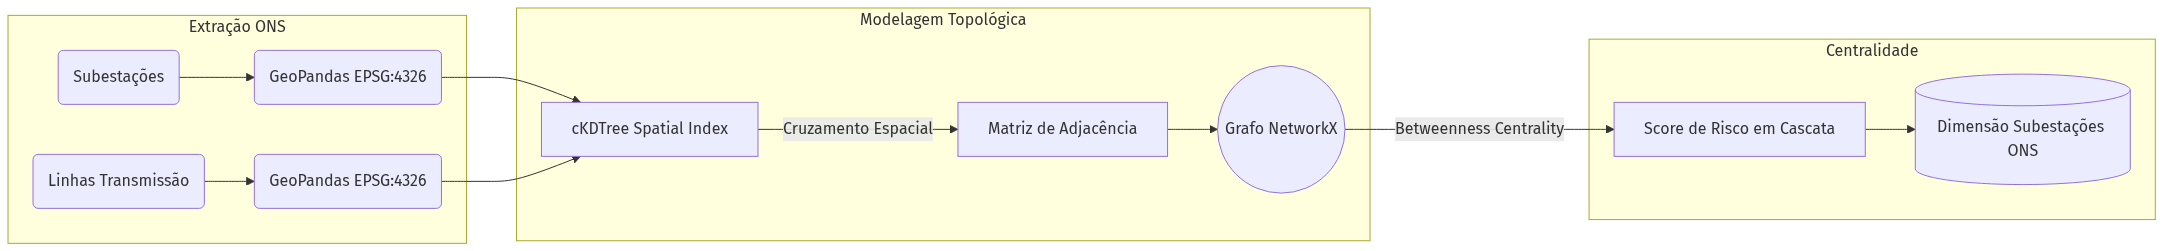
\includegraphics[width=0.9\textwidth,height=0.35\textheight,keepaspectratio]{diagrama_grafos.png}
    \caption{Modelagem Topológica de Redes via NetworkX.}
    \label{fig:grafos}
\end{figure}

Usando índices espaciais em memória (KDTrees), o sistema detecta as interseções físicas entre quilômetros de linhas de transmissão e subestações para formar uma Matriz de Adjacência. A biblioteca \textbf{NetworkX} processa o grafo e calcula a \textbf{Betweenness Centrality} de toda a rede. Esse cálculo gera um escore para cada subestação, indicando sua criticidade na transmissão e o risco de ilhamento da rede caso venha a sofrer interrupção devido a danos por queimadas em seu perímetro.

\section{Governança de IA e Engenharia de Qualidade}

Durante a evolução deste projeto, a geração de lógicas modulares ocorreu com o apoio crescente de ferramentas de Inteligência Artificial (IA) Generativa. A modernização envolveu o uso de agentes autônomos que auxiliaram na refatoração arquitetural rápida, como a conversão de formatos vetoriais (WKT para arquivos \textbf{JSON} otimizados).

No entanto, em uma arquitetura complexa, falhas de \textit{prompt} ou falta de contexto podem ocasionar poluição dos tópicos Kafka ou execução de scripts em ambientes incorretos. Para contornar esse desafio e evoluir o projeto de forma segura, adotou-se o uso de Manuais de Arquitetura (\texttt{agents.md}). 

Esses documentos funcionam como diretrizes sistêmicas (ou \textit{guardrails}) injetadas no conhecimento do agente de IA, impondo regras como: a execução imperativa via ambientes virtuais isolados (\texttt{uv run}); a proibição de alterações destrutivas na topologia do Kafka sem aviso prévio; e a priorização de testes unitários em alterações cruciais na modelagem de redes e geometria. Com isso, os benefícios da programação auxiliada por IA foram mantidos, garantindo o rigor e a segurança requeridos por projetos de dados em produção.

\section{Resultados e Discussão}

A arquitetura foi executada em ambiente local com Docker. A ingestão contínua mostrou-se estável com o Apache Druid, lidando de forma adequada com o ambiente restrito em recursos, configurando adequadamente o número de \textit{workers} e a gestão de memória.

Na avaliação do ST-DBSCAN, o sistema processou de forma eficiente uma massa bruta de milhares de focos do INPE. O algoritmo expurgou ruídos matemáticos e filtrou anomalias temporárias, conseguindo transformar coordenadas estáticas em \textbf{Eventos Dinâmicos de Incêndio}. No motor analítico, foi possível rastrear manchas de calor poligonais persistentes que ilustraram a propagação real de incêndios.

Na frente de resiliência energética, a modelagem de grafos apontou com precisão gargalos do SIN subjacentes a áreas inflamáveis. O cálculo da \textbf{Betweenness Centrality} identificou subestações que funcionam como pontes vitais entre regiões geográficas. Essa análise permite priorizar a proteção de infraestruturas que, se comprometidas pelo fogo, poderiam gerar blecautes de larga escala.

Por fim, o uso da ferramenta Dagster eliminou completamente a fragmentação dos scripts de processamento, tornando evidente o fluxo e a linhagem de ponta a ponta. 

\section{Conclusão}

Este trabalho apresentou uma arquitetura DataOps orientada a eventos, capaz de aplicar inteligência contínua a dados geoespaciais. O sistema transcende o armazenamento simples de coordenadas satelitais, evoluindo o processamento para a detecção de eventos em áreas de risco através do ST-DBSCAN e a modelagem topológica preventiva da malha elétrica utilizando a Ciência de Redes.

A separação entre orquestração, processamento de streaming em memória e o armazenamento colunar mostrou-se altamente adequada para cenários analíticos. O Dagster garantiu a rastreabilidade essencial, enquanto o Kafka e o Druid provaram escalabilidade no consumo de dados ininterruptos.

A implementação da governança explícita para agentes de IA (\texttt{agents.md}) representou um marco metodológico, garantindo que a geração de código automatizada obedeça às restrições de arquitetura de software, estabilizando e viabilizando o uso de IA no ciclo de vida de desenvolvimento do DataOps.

\section{Próximos Passos}

Para a evolução contínua da arquitetura e continuidade da pesquisa, os seguintes passos estão planejados:
\begin{itemize}
    \item \textbf{Testes de Persistência no Apache Druid}: Avaliar em profundidade a ingestão e a persistência de segmentos colunares no Apache Druid sob fluxos ininterruptos de longa duração.
    \item \textbf{Resiliência em Ambiente Docker}: Conduzir avaliações de resistência (\textit{stress tests}) e estabilidade da infraestrutura conteinerizada na máquina local, mapeando os limites de CPU e memória.
    \item \textbf{Alternativas ao Apache Superset}: Estudar a substituição ou o complemento do Apache Superset por plataformas de visualização mais especializadas, visando sanar as limitações de renderização de polígonos complexos (gerados pelo ST-DBSCAN) e painéis dinâmicos.
\end{itemize}

\section*{Declaração de Uso de Ferramentas de IA Generativa}

Durante a elaboração deste trabalho, Agentes de Inteligência Artificial Generativa foram utilizados ativamente como apoio à organização textual, revisão de trechos, estruturação de ideias, depuração de códigos, e automação na geração de diagramas (Mermaid e scripts Python). O conteúdo final, as decisões metodológicas, a validação técnica e a responsabilidade acadêmica permanecem sob total responsabilidade dos autores \cite{openai_chatgpt}.

\bibliographystyle{sbc}
\bibliography{referencias}

\end{document}
